\documentclass[11pt]{scrartcl}
\usepackage{evan}
\usepackage{mdframed}

\begin{document}
\title{A Guessing Game: When Angle A = 60 Degrees}
\author{Trung Nguyen}
\date{June 1, 2022}
\maketitle


\begin{center}
	\itshape
	Sometimes figuring out what to prove is harder than actually proving it!
\end{center}

Those of you who are familiar with Evan Chen's handouts will notice a striking resemblance between this handout and his \href{https://web.evanchen.cc/handouts/Mixt-GeoGuessr/Mixt-GeoGuessr.pdf}{Mixtilinear Incircles Guessing Game}. Indeed, I liked his idea of a Guessing Game very much that I wanted to make my own Guess Game on a different configuration. As a result, I pretty much copied the idea, structure, style sheet, etc...  (everything but the Geometry) of this handout from Evan's original Guessing Game. Huge credit goes to Evan Chen: without his work, this handout would not be possible.

In the pages that follow, I will describe a rather simple geometric configuration. It is your job to discover as many ``coincidences'' as you can: nontrivial collinearities, congruent shapes, symmetric shapes, and whatever else you can find. Can you prove your claims?

\tableofcontents

\section{The Configuration}
\begin{mdframed}
	Let $ABC$ be an acute triangle with $\angle A=60^\circ$. Let $I, O, H, N_9, I_A$ denote the 		incenter, circumcenter, orthocenter, center of the nine-point circle, and $A$-excenter of 			$\triangle ABC$, respectively. Furthermore, let $M$ be the midpoint of $\overline{II_A}$. 
\end{mdframed}

The next page contains a diagram with all these points and nothing more. There are also some hints to get you started.
However, before seeing this, \textbf{try to find as many things as you can
using your own ruler and compass.}
During a competition, one does not have access to computer-drawn diagrams!

\eject

\section{Some Hints}
Having examined the configuration with your hand-drawn diagram, try once more with a computer-generated diagram. What more can you find?

\begin{center}
	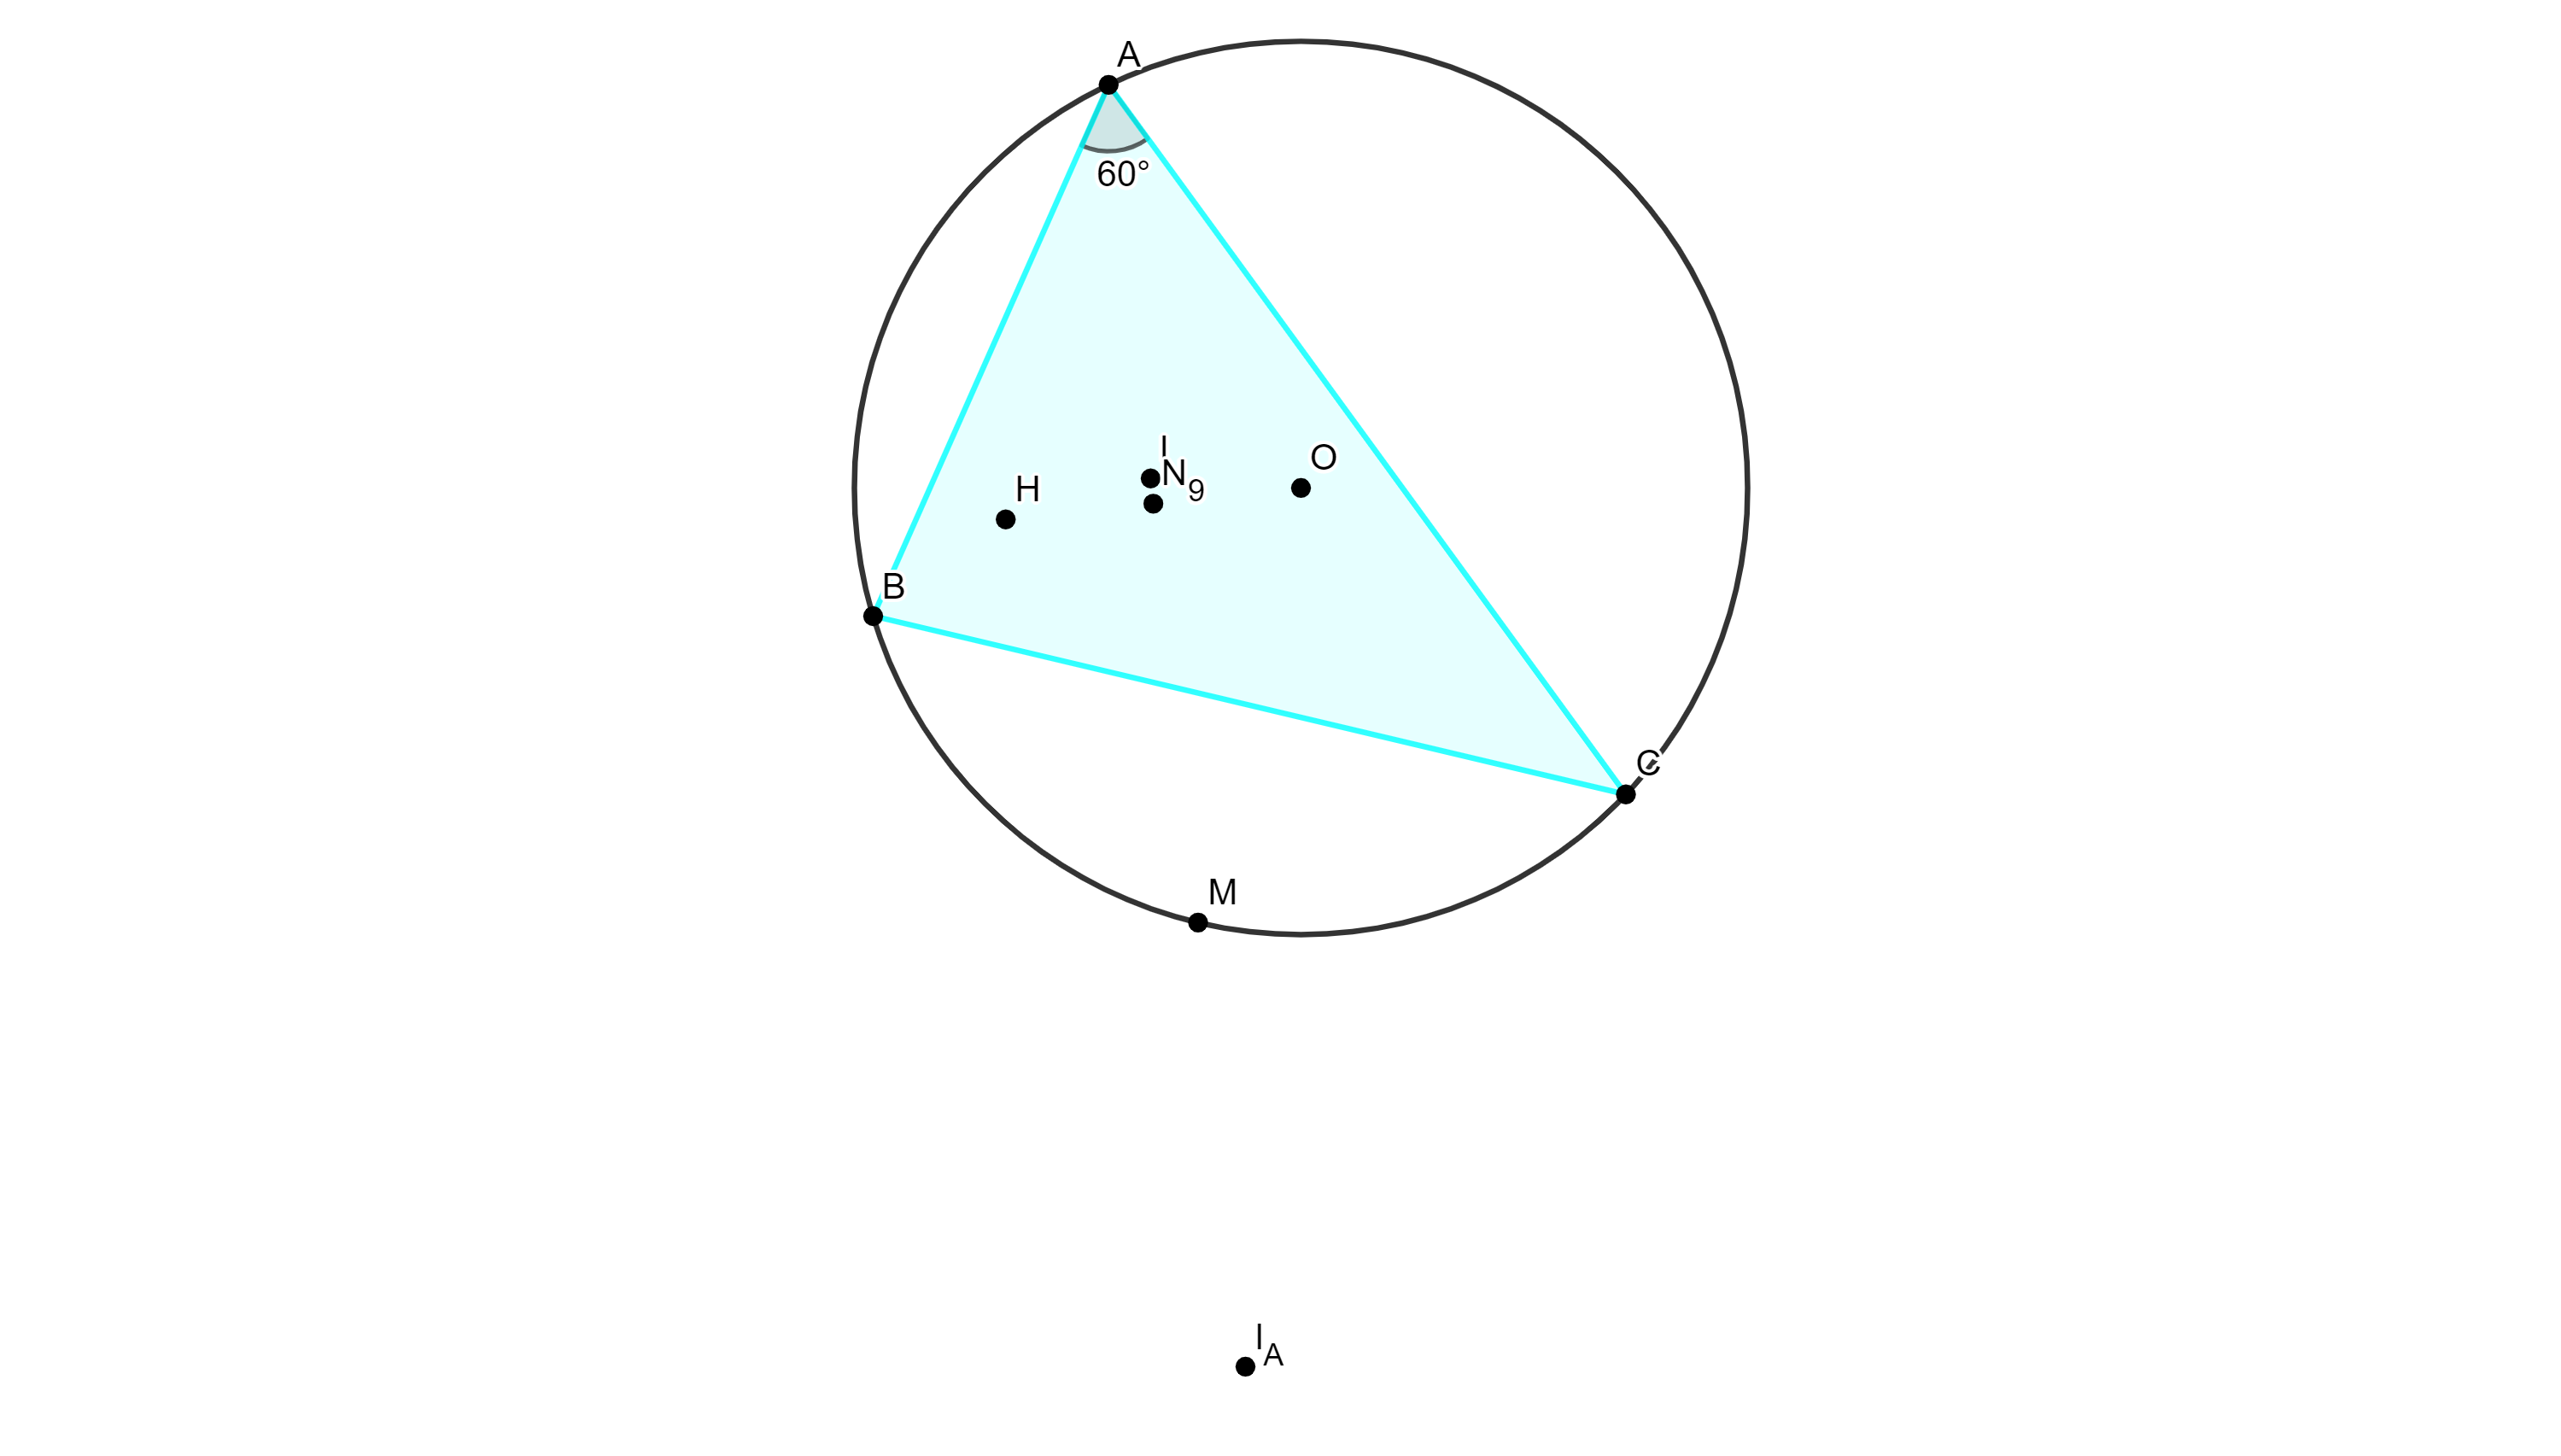
\includegraphics{A60Blank.png}
\end{center}

Here are some possible hints for things you could look for:
\begin{itemize}
	\ii A pair of congruent circles.
	\ii An equilateral triangle.
	\ii Two pairs of congruent triangles.
	\ii A cyclic hexagon.
	\ii A rhombus.
	\ii A hidden perpendicular bisector.
    \ii A (perhaps?) surprising colinearity.
\end{itemize}

My list of properties has eight items.
When you want to see my answers, turn the page.

\eject

\section{Answers}
\begin{center}
	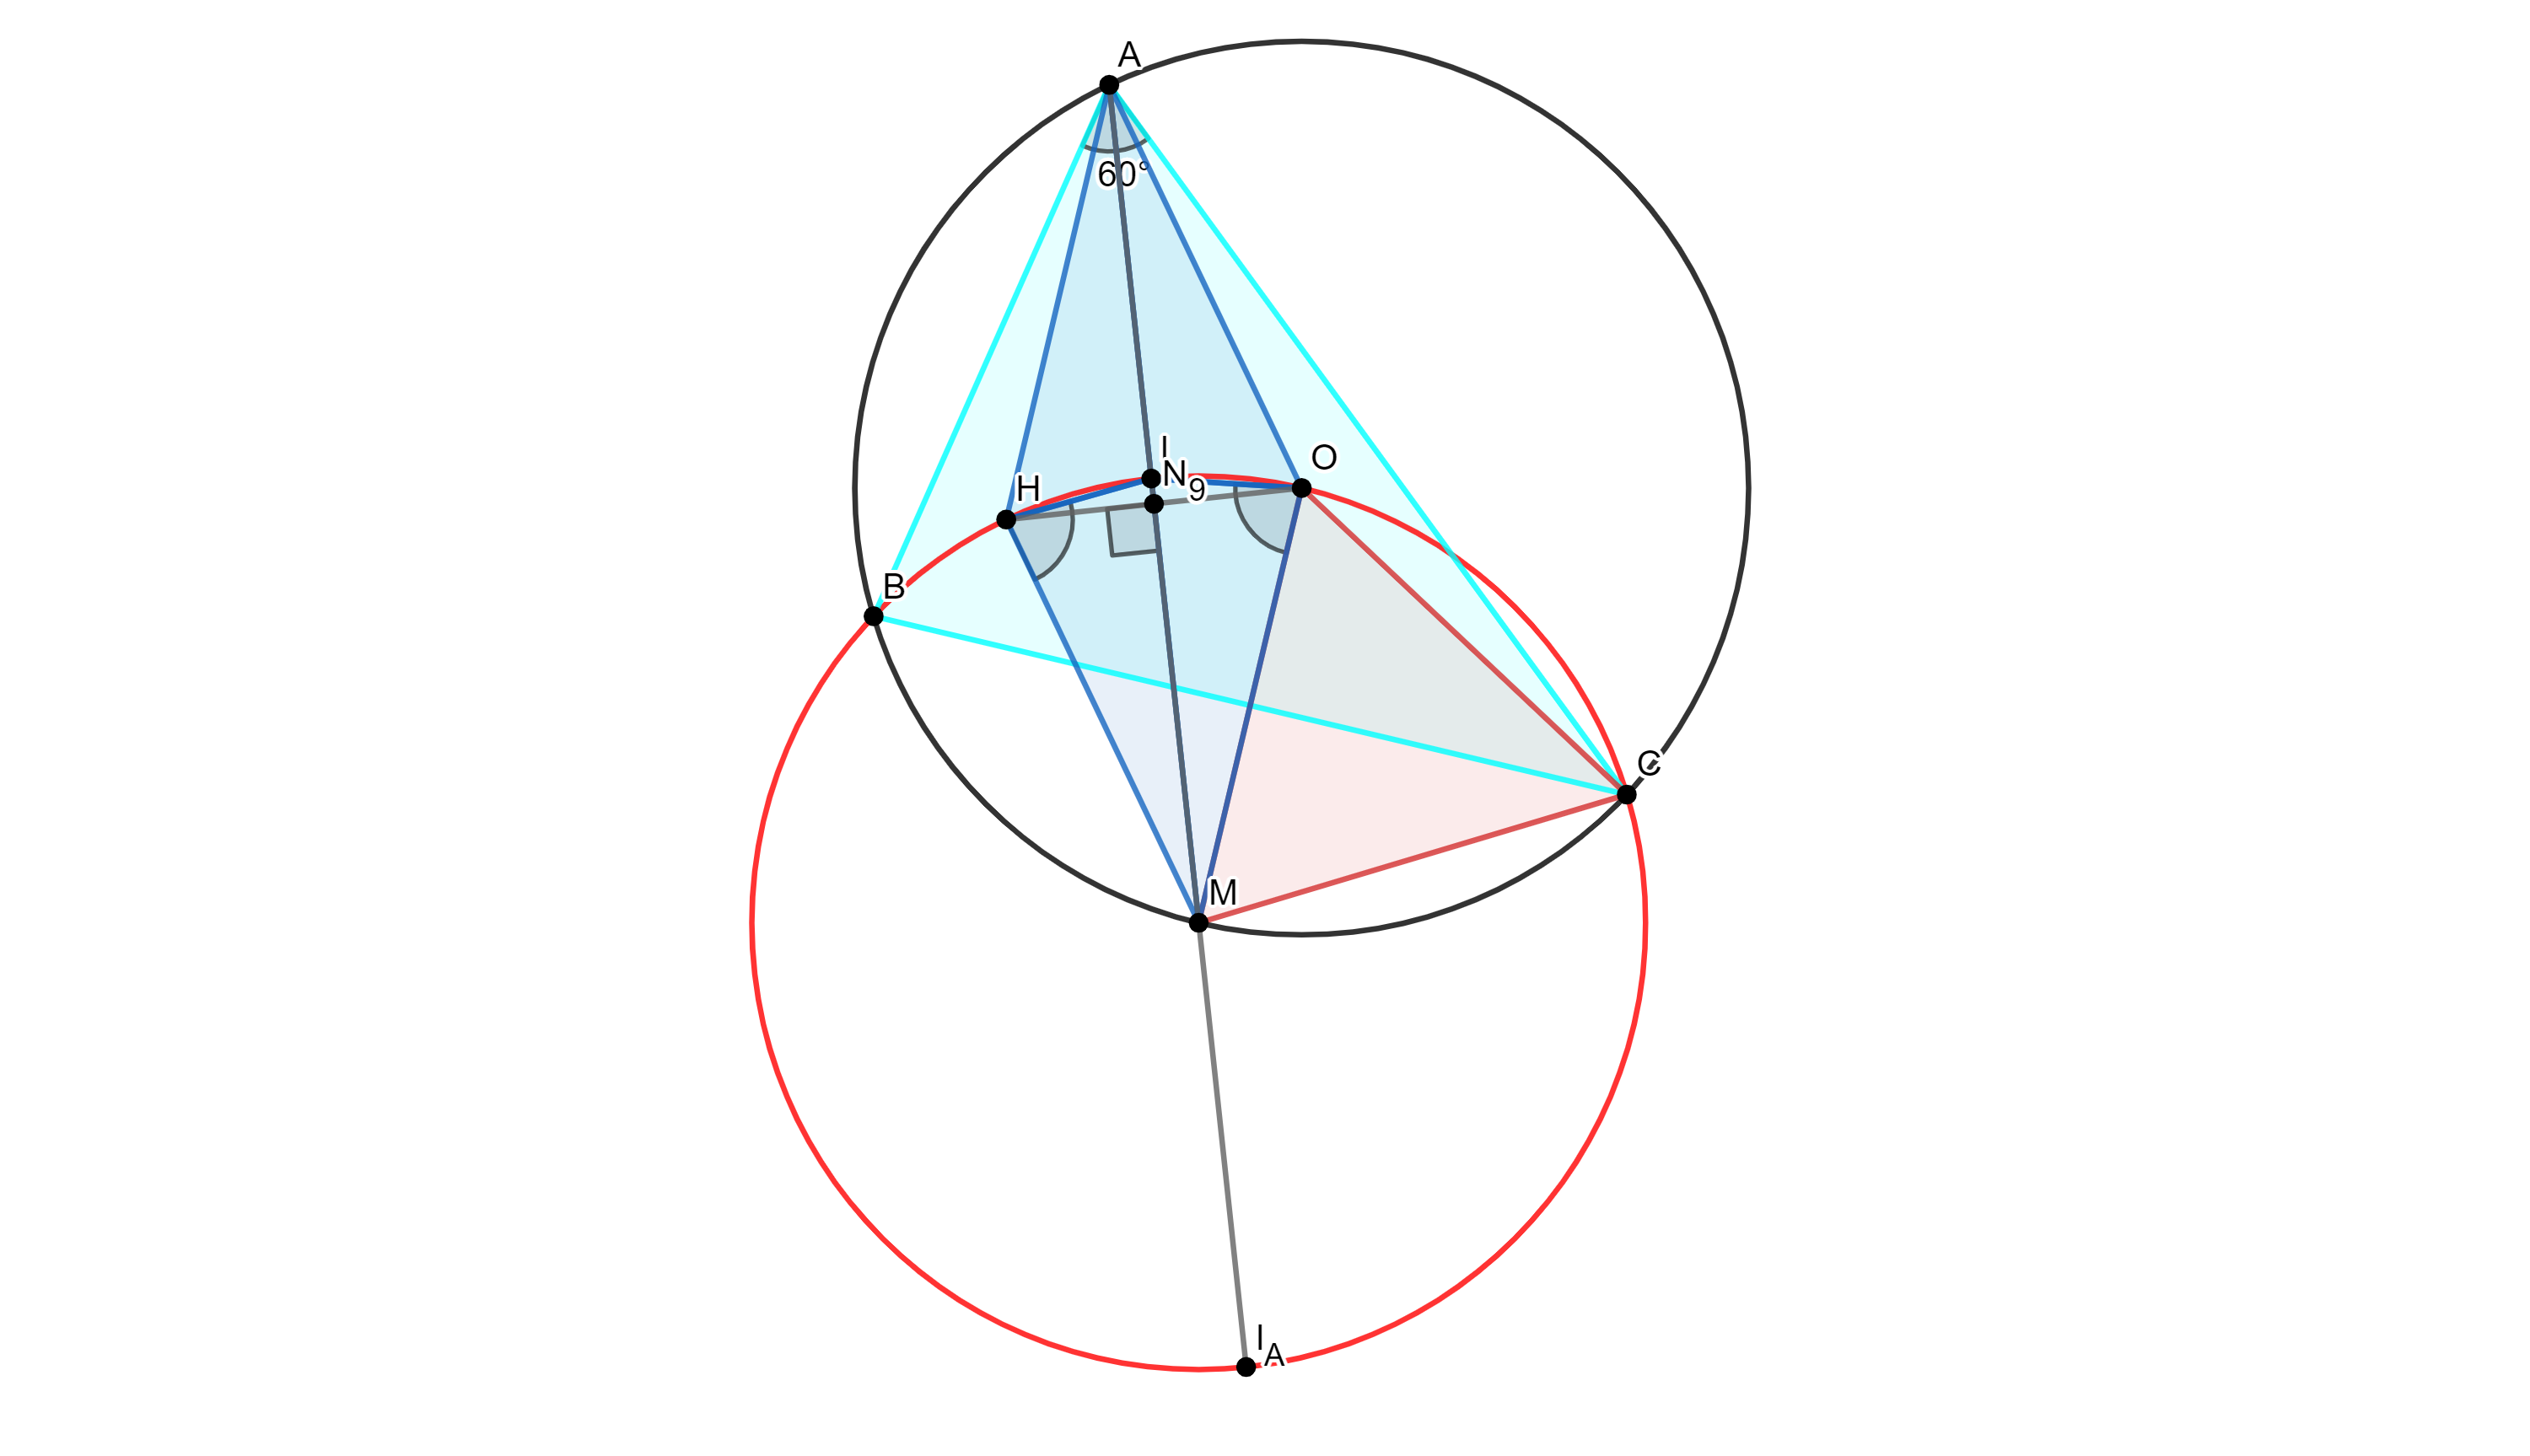
\includegraphics{A60Full.png}
\end{center}

\begin{enumerate}
	\ii $(ABC)$ and $(IBC)$ are reflections over $BC$.
	\ii $\triangle COM$ is equilateral.
	\ii $\triangle AHI\cong \triangle AOI$.
	\ii $CHIOBI_A$ is cyclic.
	\ii $\triangle IMH\cong \triangle IMO$.
	\ii $AOMH$ is a rhombus.
	\ii Line $AIM$ is the perpendicular bisector of $\overline{OH}$. 
	\ii $N_9$ lies on the line $\overline{AIM}$.
\end{enumerate}
This list is by no means exhaustive --- there are probably more properties that I just haven't mentioned.
\vspace{2em}
\section{Solutions}


These solutions freely use previously established facts to prove newer ones.
\begin{enumerate}
	\ii Denote $(ABC)$ and $(IBC)$ as $\omega_1$ and $\omega_2$ respectively. Clearly $H\in \omega_2$ and $H'\in\omega_1$ where $H'$ is the reflection of $H$ over $BC$. This is true by the Reflecting the Orthocenter Lemma. Now, for a point $P$ on $\omega_1$, we have $\measuredangle BPC=\measuredangle BAC=60^\circ$ and $\measuredangle BP'C=-\measuredangle BPC=120^\circ=\measuredangle BIC$ as needed.
    
	\ii Clearly, $IM$ bisects $\angle BIC=120^\circ$, so $\triangle MIC$ is isosceles with $\angle MIC=60^\circ$, implying the result.
    
	\ii It is well-known that $AH=2R\cos A$. Now note that $AH=2R\cos A=2R\cdot \frac12=R=AO$. Also, $AI=AI$ and $\measuredangle HAI=\measuredangle IAO$ since $H$ and $O$ are isogonal conjugates. Thus, $\triangle AHI\cong \triangle AOI$.
    
	\ii Observe the following angle equalities:\begin{align*} \angle BHC&=180^\circ-\angle A=120^\circ\\ \angle BIC&=90^\circ+\frac{\angle A}2=120^\circ\\ \angle BOC&=2\angle A=120^\circ \end{align*}
so hexagon $CHIOBI_A$ is cyclic.

	\ii We have $MH=MO$ and $MI=MI$. Also note that $\measuredangle HMI=\measuredangle IMO$ since $H$ and $O$ are isogonal conjugates and thus reflections across the line $\overline{AIM}$. Thus $\triangle IMH\cong \triangle IMO$.
    
	\ii Observe that $AH\parallel OM$. From the above, we have $MH=MO=AO=AH$, finishing. (Actually, the parallel condition was not even needed.)
    
	\ii This follows from $AO=AH$ (or $MH=MO$) combined with the $O$ and $H$ isogonality.
    
	\ii $N_9$ is the midpoint of $\overline{OH}$ which does the trick.
\end{enumerate}
\vspace{18em}

\section{Problems}
Now that you are an expert at this configuration, try some problems!


\begin{enumerate}
	\ii In $\triangle ABC$, points $D$ and $E$ are constructed on sides $BC$ and $CA$ such that $AD$ and $BE$ are angle bisectors. Prove that $\angle ACB = 60^\circ$ if and only if $AE + BD = AB$. (\href{https://artofproblemsolving.com/community/c4h2260732p17495718}{2016 Kyiv City MO} and \href{https://artofproblemsolving.com/community/c6h2402244p19698819}{2017 Saint Petersburg State University School Olympiad})
    

    
    
	\ii In $\triangle ABC,$ let $\angle B = 60^\circ$, $O$ denote the circumcenter, and $L$ denote the foot of the $B$-angle bisector. The circumcirle of triangle $BOL$ meets the circumcircle of $ABC$ at point $D \ne B$. Prove that $BD \perp AC$. (\href{https://artofproblemsolving.com/community/c6h2259561p17475948}{2019 Saudi Arabia IMO Training Test 3.1})

    
    
    
	\ii In $\triangle ABC$, $AB>AC$. Let $O$ and $I$ be the circumcenter and incenter respectively. Prove that if $\angle AIO = 30^{\circ}$, then $\angle ABC = 60^{\circ}$. (\href{https://artofproblemsolving.com/community/c6h2220657p16878510}{2020 China North Mathematical Olympiad Advanced Level P2})
    
    
	\ii In $\triangle ABC$, let $O$ denote the circumcenter and $H$ denote the orthocenter. Prove that $\angle A=60^\circ$ if (a) $AO=AH$ or if (b) quadrilateral $BOCH$ is cyclic. (\href{https://artofproblemsolving.com/community/c4h2060529p14687121}{AoPS Forums})
    
    
	\ii In $\triangle ABC$, angle $\angle B=60^\circ$. Points $D$ and $E$ are constructed on sides $BC$ and $CA$ such that $AD$ and $BE$ are angle bisectors. If $O$ is the incenter, prove that $OD=OE$. (\href{https://artofproblemsolving.com/community/c4h2133091p15607072}{AoPS Forums})
    
    
    
	\ii In non-isosceles $\triangle ABC$ with $\angle ABC=60$, a point $T$ in its interior is selected such that $\angle ATC=\angle BTC=\angle BTA=120^\circ$. Let $M$ be the intersection point of the medians in $\triangle ABC$ and let $TM$ intersect $(ATC)$ at $K$. Find $\frac{TM}{MK}$. (\href{https://artofproblemsolving.com/community/c6h2535040}{2021 ARO 9.6})
    
    
    
	\ii Let $ABC$ be an acute angled triangle with $\angle{BAC}=60^\circ$ and $AB > AC$. Let $I$ be the incenter, and $H$ the orthocenter of the triangle $ABC$ . Prove that $2\angle{AHI}= 3\angle{ABC}$. (\href{https://artofproblemsolving.com/community/c6h141391p799589}{2007 APMO})
    
    
	\ii Suppose $\triangle ABC$ has orthocenter $F$, incenter $E$ and circumcenter $D$. Find all angles $\angle B$ such that $AFED$ is a cyclic quadrilateral. (\href{hhttps://artofproblemsolving.com/community/c4h2537747p21610688}{AoPS Forums})


	\ii Let $\triangle ABC$ be acute with $\angle A = 60^\circ$. Prove that $IH = IO$, where $I, H, O$ denote the incenter, orthocenter, and circumcenter, respectively. (\href{https://artofproblemsolving.com/community/c6h1408296}{AoPS Forums})


	\ii Triangle $ABC$ has $\angle BAC=60^\circ$, $\angle CBA \le 90^\circ$, $BC=1$, and $AC \ge AB$. Let $H$, $I$, and $O$ be the orthocenter, incenter, and circumcenter of $\triangle ABC$, respectively. Assume that the area of the pentagon $BCOIH$ is the maximum possible. What is $\angle CBA$?(\href{https://artofproblemsolving.com/community/c5h390791}{2011 AMC 12A Problem 25})

	\ii Let $ABC$ be a scalene triangle with $\angle A = 60^{\circ}$. Let $E$ and $F$ be the feet of the angle bisectors of $\angle ABC$ and $\angle ACB$, respectively, and let $I$ be the incenter of $\triangle ABC$. Let $P,Q$ be distinct points such that $\triangle PEF$ and $\triangle QEF$ are equilateral. If $O$ is the circumcenter of of $\triangle APQ$, show that $\overline{OI}\perp \overline{BC}$. (\href{https://artofproblemsolving.com/community/c6h1472056}{2017 ELMO SL G2})
    
\end{enumerate}



\end{document}